\documentclass[11pt]{article}
\usepackage[margin=1in]{geometry}
\usepackage{amsmath,amssymb,booktabs,array,longtable}
\usepackage{graphicx}
\usepackage{tikz}
\usetikzlibrary{shapes.geometric, arrows, positioning}
\usepackage{hyperref}
\usepackage{enumitem}
\usepackage{titlesec}
\usepackage{float}

\begin{document}

\begin{center}
\Large\textbf{Shiv Nadar University Chennai}\\
\end{center}

\begin{center}
\textbf{CS3807 – Deep Learning Laboratory}
\vspace{2mm}

\textbf{Experiment 4}
\vspace{2mm}

\textbf{Comparative Study of Deep Convolutional Neural Network Architectures Using Transfer Learning}
\end{center}

\renewcommand{\arraystretch}{1.4}

\begin{tabular}{|p{3.5cm}|p{8cm}|p{2cm}|}
\hline
Degree \& Branch & B.Tech Artificial Intelligence \& Data Science & Semester V\\ \hline
Subject Code \& Name & CS3807 -- Deep Learning Laboratory & AY: 2026--27\\ \hline
\end{tabular}
\vspace{3mm}

\section{Objective}
The objectives of this experiment are:
\begin{itemize}[leftmargin=*]
    \item Study the evolution of deep CNN architectures.
    \item Compare LeNet-5, AlexNet, VGG16, GoogleNet, and ResNet.
    \item Understand transfer learning.
    \item Fine tune pretrained CNN models.
    \item Compare classification performance of different architectures.
\end{itemize}

\section{Learning Outcomes}
After completing this experiment students will be able to:
\begin{enumerate}[leftmargin=*]
    \item Explain modern CNN architectures.
    \item Differentiate LeNet, AlexNet, VGG16, GoogleNet, and ResNet.
    \item Implement transfer learning.
    \item Fine tune pretrained CNN models.
    \item Compare CNN architectures using performance metrics.
\end{enumerate}

\section{Introduction}
Deep Convolutional Neural Networks have become the dominant models for computer vision applications because they automatically learn hierarchical features from images. The evolution of CNNs has focused on improving classification accuracy while reducing computational complexity and training difficulties.

The progression of CNN architectures began with LeNet-5 and has evolved through AlexNet, VGGNet, GoogleNet, and ResNet. Each architecture introduced important innovations that significantly improved image classification performance.

\section{Evolution of CNN Architectures}
\begin{table}[H]
\centering
\begin{tabular}{|l|l|p{8cm}|}
\hline
\textbf{Model} & \textbf{Year} & \textbf{Major Contribution} \\ \hline
LeNet-5 & 1998 & First practical convolutional neural network \\ \hline
AlexNet & 2012 & ReLU activation, Dropout and GPU training \\ \hline
VGG16 & 2014 & Uniform $3 \times 3$ convolution filters \\ \hline
GoogleNet & 2014 & Inception modules for multi-scale feature extraction \\ \hline
ResNet & 2015 & Residual learning using skip connections \\ \hline
\end{tabular}
\end{table}

\section{LeNet-5}
LeNet-5 was proposed by Yann LeCun in 1998 for handwritten digit recognition. It consists of two convolution layers, two average pooling layers, and fully connected layers. It demonstrated that convolutional networks could automatically learn image features without handcrafted feature extraction.

\paragraph{Advantages}
\begin{itemize}[leftmargin=*]
    \item Small number of parameters
    \item Fast training
    \item Suitable for OCR
\end{itemize}

\section{AlexNet}
AlexNet won the ImageNet Challenge in 2012 by reducing the classification error significantly. It introduced ReLU activation, Dropout regularization, and GPU training.

\paragraph{Major Innovations}
\begin{itemize}[leftmargin=*]
    \item ReLU activation
    \item Dropout
    \item GPU implementation
    \item Data augmentation
\end{itemize}

\section{VGG16}
VGG16 demonstrated that using multiple small $3 \times 3$ convolution filters could outperform larger filters while increasing network depth.

\paragraph{Advantages}
\begin{itemize}[leftmargin=*]
    \item Excellent feature extraction
    \item Simple architecture
    \item High classification accuracy
\end{itemize}

\section{Comparison of Architectures}
\begin{table}[H]
\centering
\begin{tabular}{|l|l|l|p{6cm}|}
\hline
\textbf{Architecture} & \textbf{Depth} & \textbf{Parameters} & \textbf{Main Contribution} \\ \hline
LeNet-5 & 7 & 60K & First CNN \\ \hline
AlexNet & 8 & 61M & ReLU + Dropout \\ \hline
VGG16 & 16 & 138M & Deep $3 \times 3$ filters \\ \hline
GoogleNet & 22 & 6.8M & Inception Modules \\ \hline
ResNet50 & 50 & 25.6M & Residual Learning \\ \hline
\end{tabular}
\end{table}

\section{GoogleNet (Inception Network)}
GoogleNet, proposed by Szegedy et al. in 2014, introduced the Inception Module, which performs multiple convolution operations in parallel using different filter sizes. Instead of using only a single kernel size, GoogleNet simultaneously applies $1 \times 1$, $3 \times 3$, $5 \times 5$ convolutions and max pooling. The outputs are concatenated to obtain multi-scale feature representations.

The use of $1 \times 1$ convolutions before larger kernels reduces the number of trainable parameters and computational complexity.

\paragraph{Advantages}
\begin{itemize}[leftmargin=*]
    \item Multi-scale feature extraction.
    \item Fewer parameters than VGG16.
    \item High computational efficiency.
    \item Better classification performance.
\end{itemize}
\newpage
\section{ResNet}
Increasing CNN depth often causes the vanishing gradient problem, making optimization difficult. ResNet solves this issue using skip (residual) connections, allowing gradients to flow directly through the network.

Instead of learning 
\[
H(x)
\], 

ResNet learns:
\[
F(x) = H(x) - x
\]

thus,
\[
\text{Output} = F(x) + x
\]
where:
\begin{itemize}[leftmargin=*]
    \item $F(x) = \text{Residual Mapping}$
    \item $x = \text{Identity Mapping}$
\end{itemize}

\begin{figure}[H]
\centering
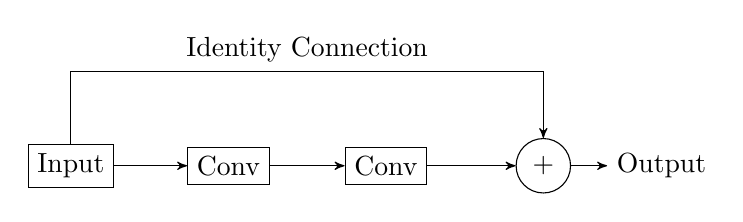
\begin{tikzpicture}[node distance=1.5cm, auto, >=stealth']
    % Fixed: Added (input) node name before the label
    \node [draw, rectangle] (input) {Input};
    \node [draw, rectangle, right of=input, node distance=2cm] (conv1) {Conv};
    \node [draw, rectangle, right of=conv1, node distance=2cm] (conv2) {Conv};
    \node [draw, circle, right of=conv2, node distance=2cm] (add) {$+$};
    \node [right of=add, node distance=1.5cm] (output) {Output};

    % Straight flow connections
    \draw[->] (input) -- (conv1);
    \draw[->] (conv1) -- (conv2);
    \draw[->] (conv2) -- (add);
    \draw[->] (add) -- (output);
    
    % Fixed: Identity connection pathing
    \draw[->] (input) |- ++(0,1.2) -| node[near start, above] {Identity Connection} (add);
\end{tikzpicture}
\caption{Residual Block in ResNet}
\label{fig:residual_block}
\end{figure}

\paragraph{Advantages}
\begin{itemize}[leftmargin=*]
    \item Eliminates vanishing gradients.
    \item Enables very deep neural networks.
    \item Faster convergence.
    \item High ImageNet accuracy.
\end{itemize}

\section{Dilated Convolution}
Dilated convolution (also called atrous convolution) increases the receptive field without increasing the number of parameters. The dilation rate determines the spacing between kernel elements.

For a standard convolution:
\[
D = 1
\]
For dilated convolution:
\[
D > 1
\]

\paragraph{Example}
\[
\begin{bmatrix}
1 & 0 & 2 \\
0 & 3 & 0 \\
4 & 0 & 5
\end{bmatrix}
\]
where zeros indicate inserted gaps.

\paragraph{Applications}
\begin{itemize}[leftmargin=*]
    \item Semantic segmentation
    \item Medical image analysis
    \item Satellite imagery
    \item Object localization
\end{itemize}

\section{Transpose Convolution}
Transpose convolution increases the spatial dimensions of feature maps. Unlike pooling, which reduces image size, transpose convolution performs learnable upsampling.

\paragraph{Applications}
\begin{itemize}[leftmargin=*]
    \item Image Super Resolution
    \item Autoencoders
    \item GANs
    \item Image Generation
    \item Semantic Segmentation
\end{itemize}

\section{Transfer Learning}
Transfer Learning utilizes a pretrained CNN model that has already learned general image features from a large dataset such as ImageNet.

Instead of training from scratch:
\begin{enumerate}[leftmargin=*]
    \item Load a pretrained model.
    \item Remove the original classifier.
    \item Freeze convolution layers.
    \item Add new Dense layers.
    \item Train the classifier.
    \item Fine tune selected convolution layers.
\end{enumerate}

\begin{figure}[H]
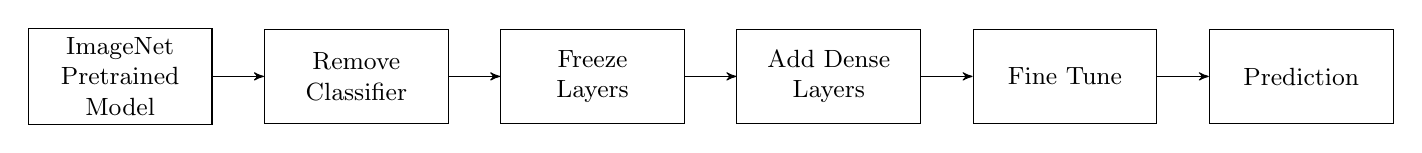
\begin{tikzpicture}[node distance=3cm, auto, >=stealth', block/.style={draw, rectangle, align=center, minimum height=1.2cm, text width=2.1cm, font=\small}]
    \node [block] (b1) {ImageNet\\Pretrained Model};
    \node [block, right of=b1] (b2) {Remove\\Classifier};
    \node [block, right of=b2] (b3) {Freeze\\Layers};
    \node [block, right of=b3] (b4) {Add Dense\\Layers};
    \node [block, right of=b4] (b5) {Fine Tune};
    \node [block, right of=b5] (out) {Prediction};

    \draw[->] (b1.east) -- (b2.west);
    \draw[->] (b2.east) -- (b3.west);
    \draw[->] (b3.east) -- (b4.west);
    \draw[->] (b4.east) -- (b5.west);
    \draw[->] (b5.east) -- (out.west);
\end{tikzpicture}
\caption{Transfer Learning Workflow}
\label{fig:transfer_learning}
\end{figure}

\paragraph{Advantages}
\begin{itemize}[leftmargin=*]
    \item Faster convergence.
    \item Higher accuracy on small datasets.
    \item Reduced training time.
    \item Lower computational cost.
\end{itemize}

\section{Dataset}
\textbf{Dataset: CIFAR-10}
\begin{itemize}[leftmargin=*]
    \item Training Images: 50,000
    \item Testing Images: 10,000
    \item Number of Classes: 10
    \item Image Size: $32 \times 32 \times 3$
    \item Classes: Airplane, Automobile, Bird, Cat, Deer, Dog, Frog, Horse, Ship, and Truck.
\end{itemize}

\section{Experimental Procedure}
\paragraph{Task 1: Dataset Preparation}
\begin{enumerate}
    \item Load the CIFAR-10 dataset using TensorFlow/Keras.
    \item Normalize the pixel values to the range $[0, 1]$.
    \item Display ten sample images.
    \item Print the dimensions of the training and testing datasets.
\end{enumerate}

\paragraph{Task 2: Transfer Learning}\hfill\\
Load any one of the following pretrained CNN models:
\begin{itemize}
    \item VGG16
    \item ResNet50
    \item MobileNetV2
    \item EfficientNetB0 (Optional)
\end{itemize}
Perform the following steps:
\begin{enumerate}
    \item Load pretrained ImageNet weights.
    \item Remove the original classification layer.
    \item Freeze the convolutional base.
    \item Add a Global Average Pooling layer.
    \item Add a Dense layer with ReLU activation.
    \item Add the output layer with Softmax activation.
\end{enumerate}

\paragraph{Task 3: Model Training}\hfill\\
Train the model using:
\begin{table}[H]
\centering
\begin{tabular}{|l|l|}
\hline
\textbf{Hyperparameter} & \textbf{Value} \\ \hline
Optimizer & Adam \\ \hline
Learning Rate & 0.001 \\ \hline
Batch Size & 32 \\ \hline
Epochs & 10–20 \\ \hline
Loss Function & Categorical Cross Entropy \\ \hline
Evaluation Metric & Accuracy \\ \hline
\end{tabular}
\end{table}

\paragraph{Task 4: Fine Tuning}
\begin{enumerate}
    \item Unfreeze the last convolution block.
    \item Train for another 5–10 epochs.
    \item Compare the classification accuracy before and after fine-tuning.
\end{enumerate}

\paragraph{Task 5: Model Evaluation}\hfill\\
Evaluate the trained model using:
\begin{itemize}
    \item Accuracy
    \item Precision
    \item Recall
    \item F1-score
    \item Confusion Matrix
    \item Classification Report
\end{itemize}

\section{Hyperparameter Study}
Compare the performance using different settings.

\begin{table}[H]
\centering
\begin{tabular}{|l|l|}
\hline
\textbf{Hyperparameter} & \textbf{Values} \\ \hline
Learning Rate & 0.001, 0.0001 \\ \hline
Batch Size & 16, 32, 64 \\ \hline
Epochs & 10, 20 \\ \hline
Optimizer & Adam, SGD \\ \hline
Dense Units & 128, 256 \\ \hline
Frozen Layers & All, Partial \\ \hline
\end{tabular}
\end{table}

\section{Source Code}
\noindent\textbf{Source:} Github\\
\noindent\textbf{Github Repository Link:}

\url{https://github.com/ssvibitha/DeepLearningLab_2026-27/blob/main/Lab4_TransferLearning/DL_Lab4.ipynb}


\section{Plots and Inference}
\begin{enumerate}
    \item\textbf{Sample CIFAR-10 images}
        \begin{figure}[H]
        \centering
        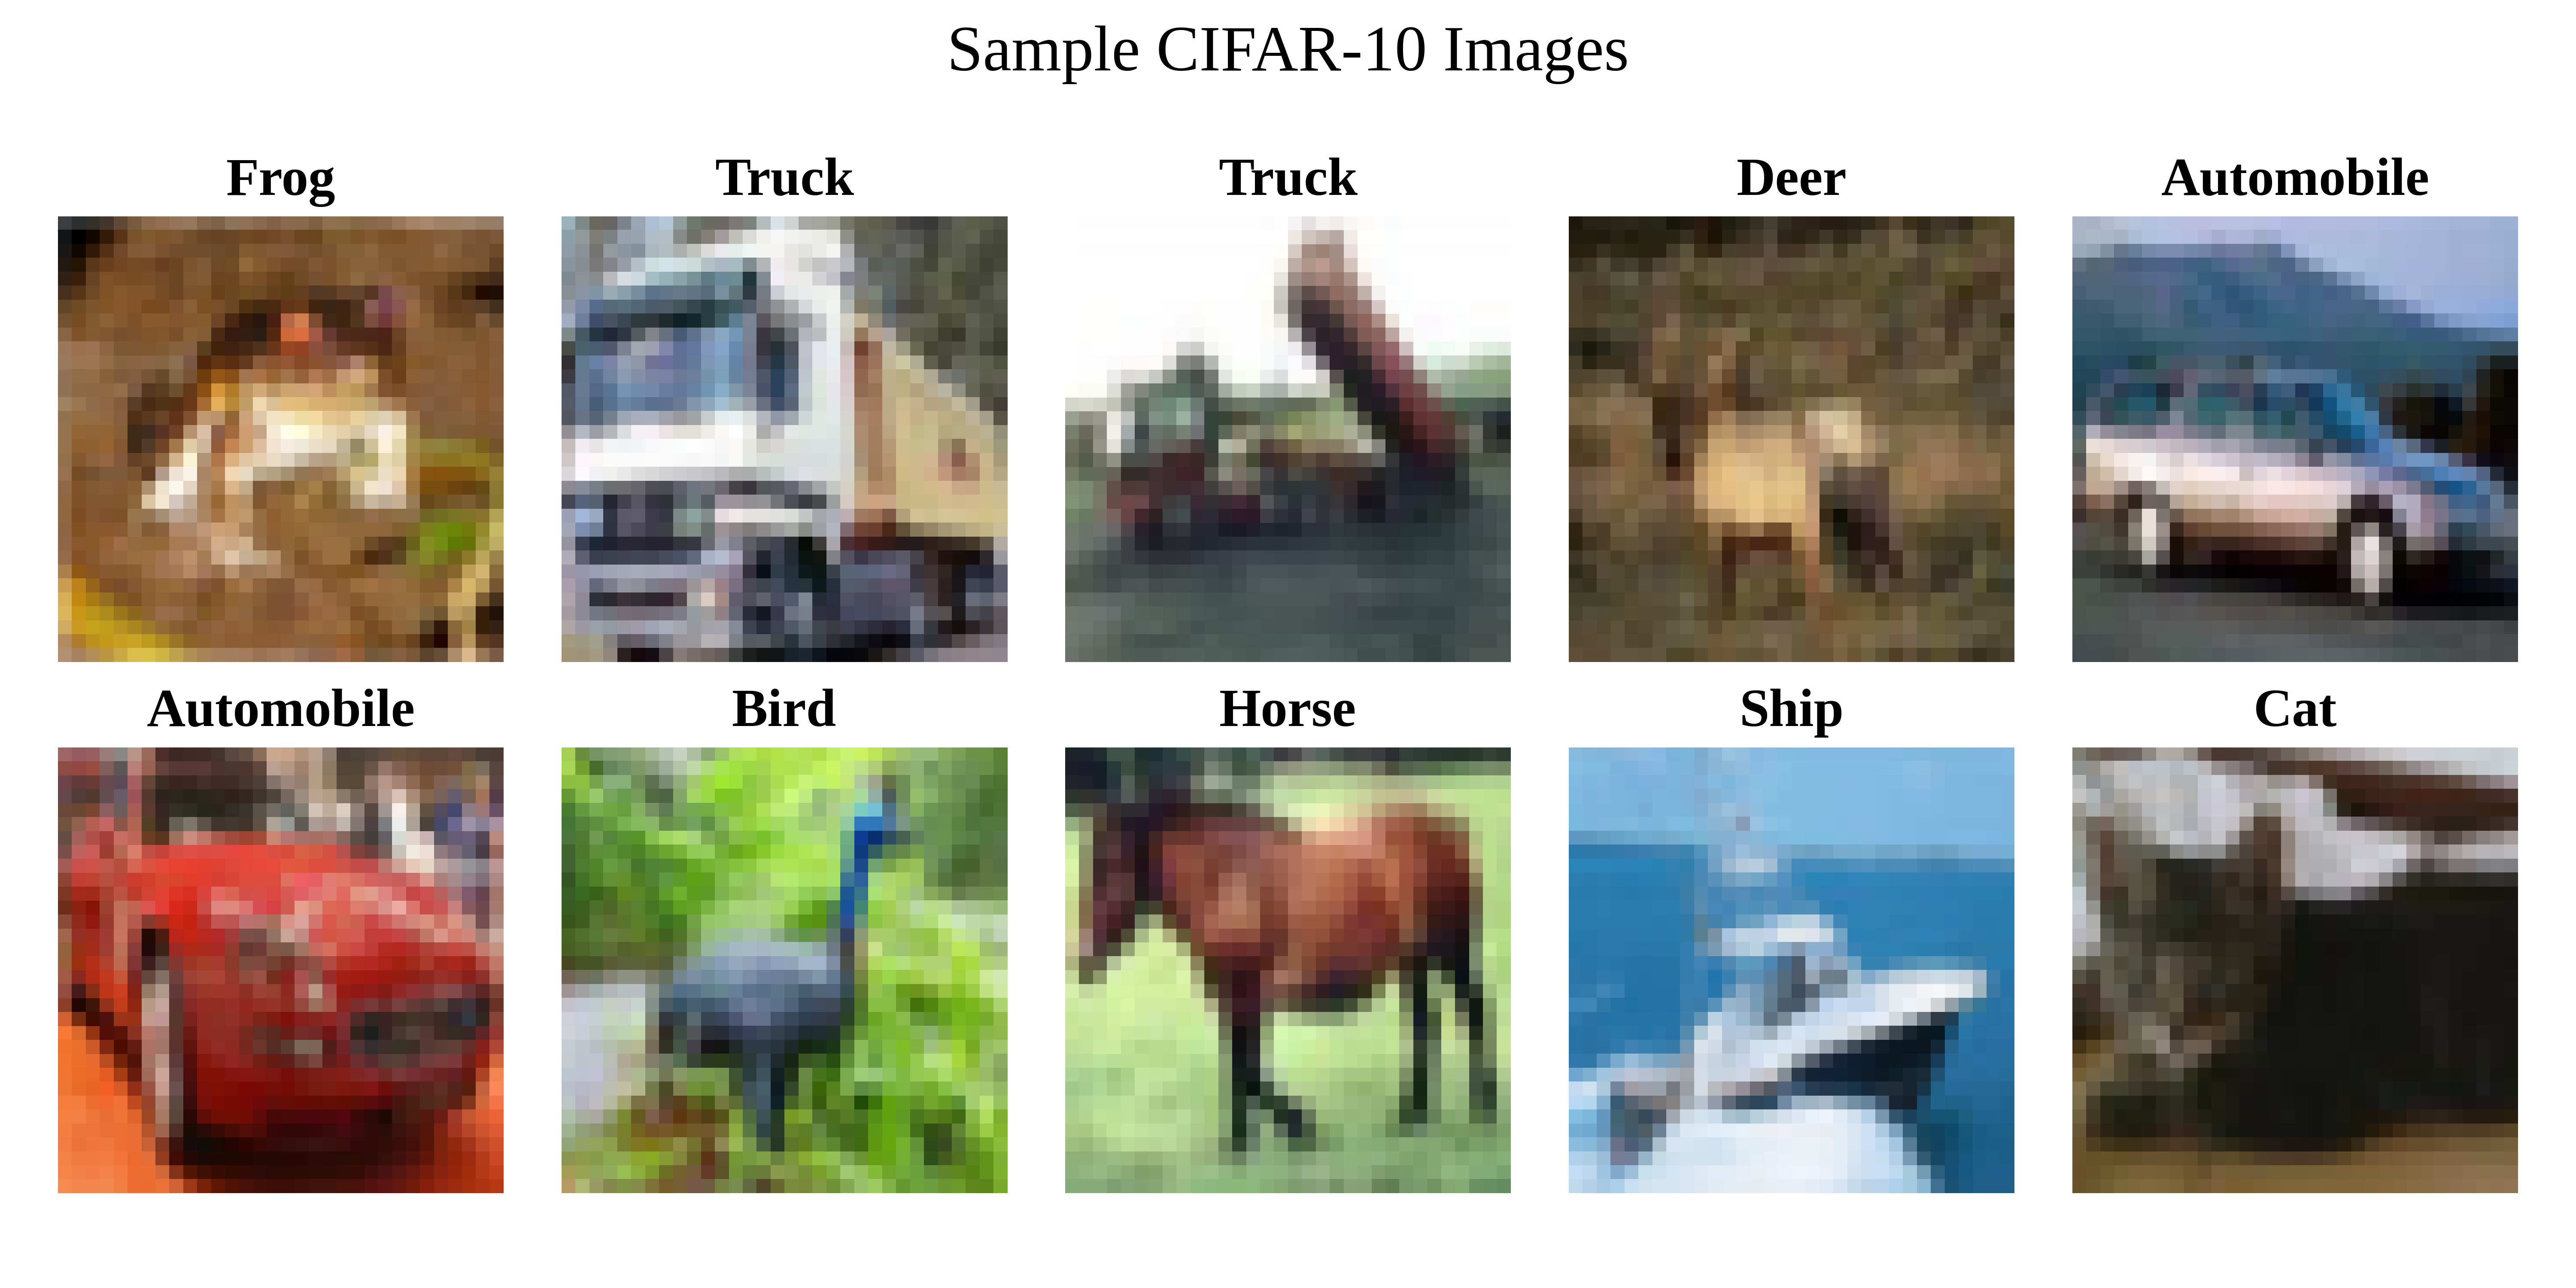
\includegraphics[width=0.8\textwidth]{Images/SampleImages.png}
        \caption{Sample Images}
        \label{fig:SampleImages}
    \end{figure}
    \noindent\textbf{Inference:}\\
    The figures show sample images from the CIFAR-10 dataset. 
    The images belong to 10 different categories such as Airplane, Automobile, Bird, Cat, Deer, Dog, Frog, Horse, Ship and Truck.
    Each image is 32 x 32 pixels and contains three color channels (RGB)
    
    
    \item\textbf{Training and Validation Accuracy}
            \begin{figure}[H]
            \centering
            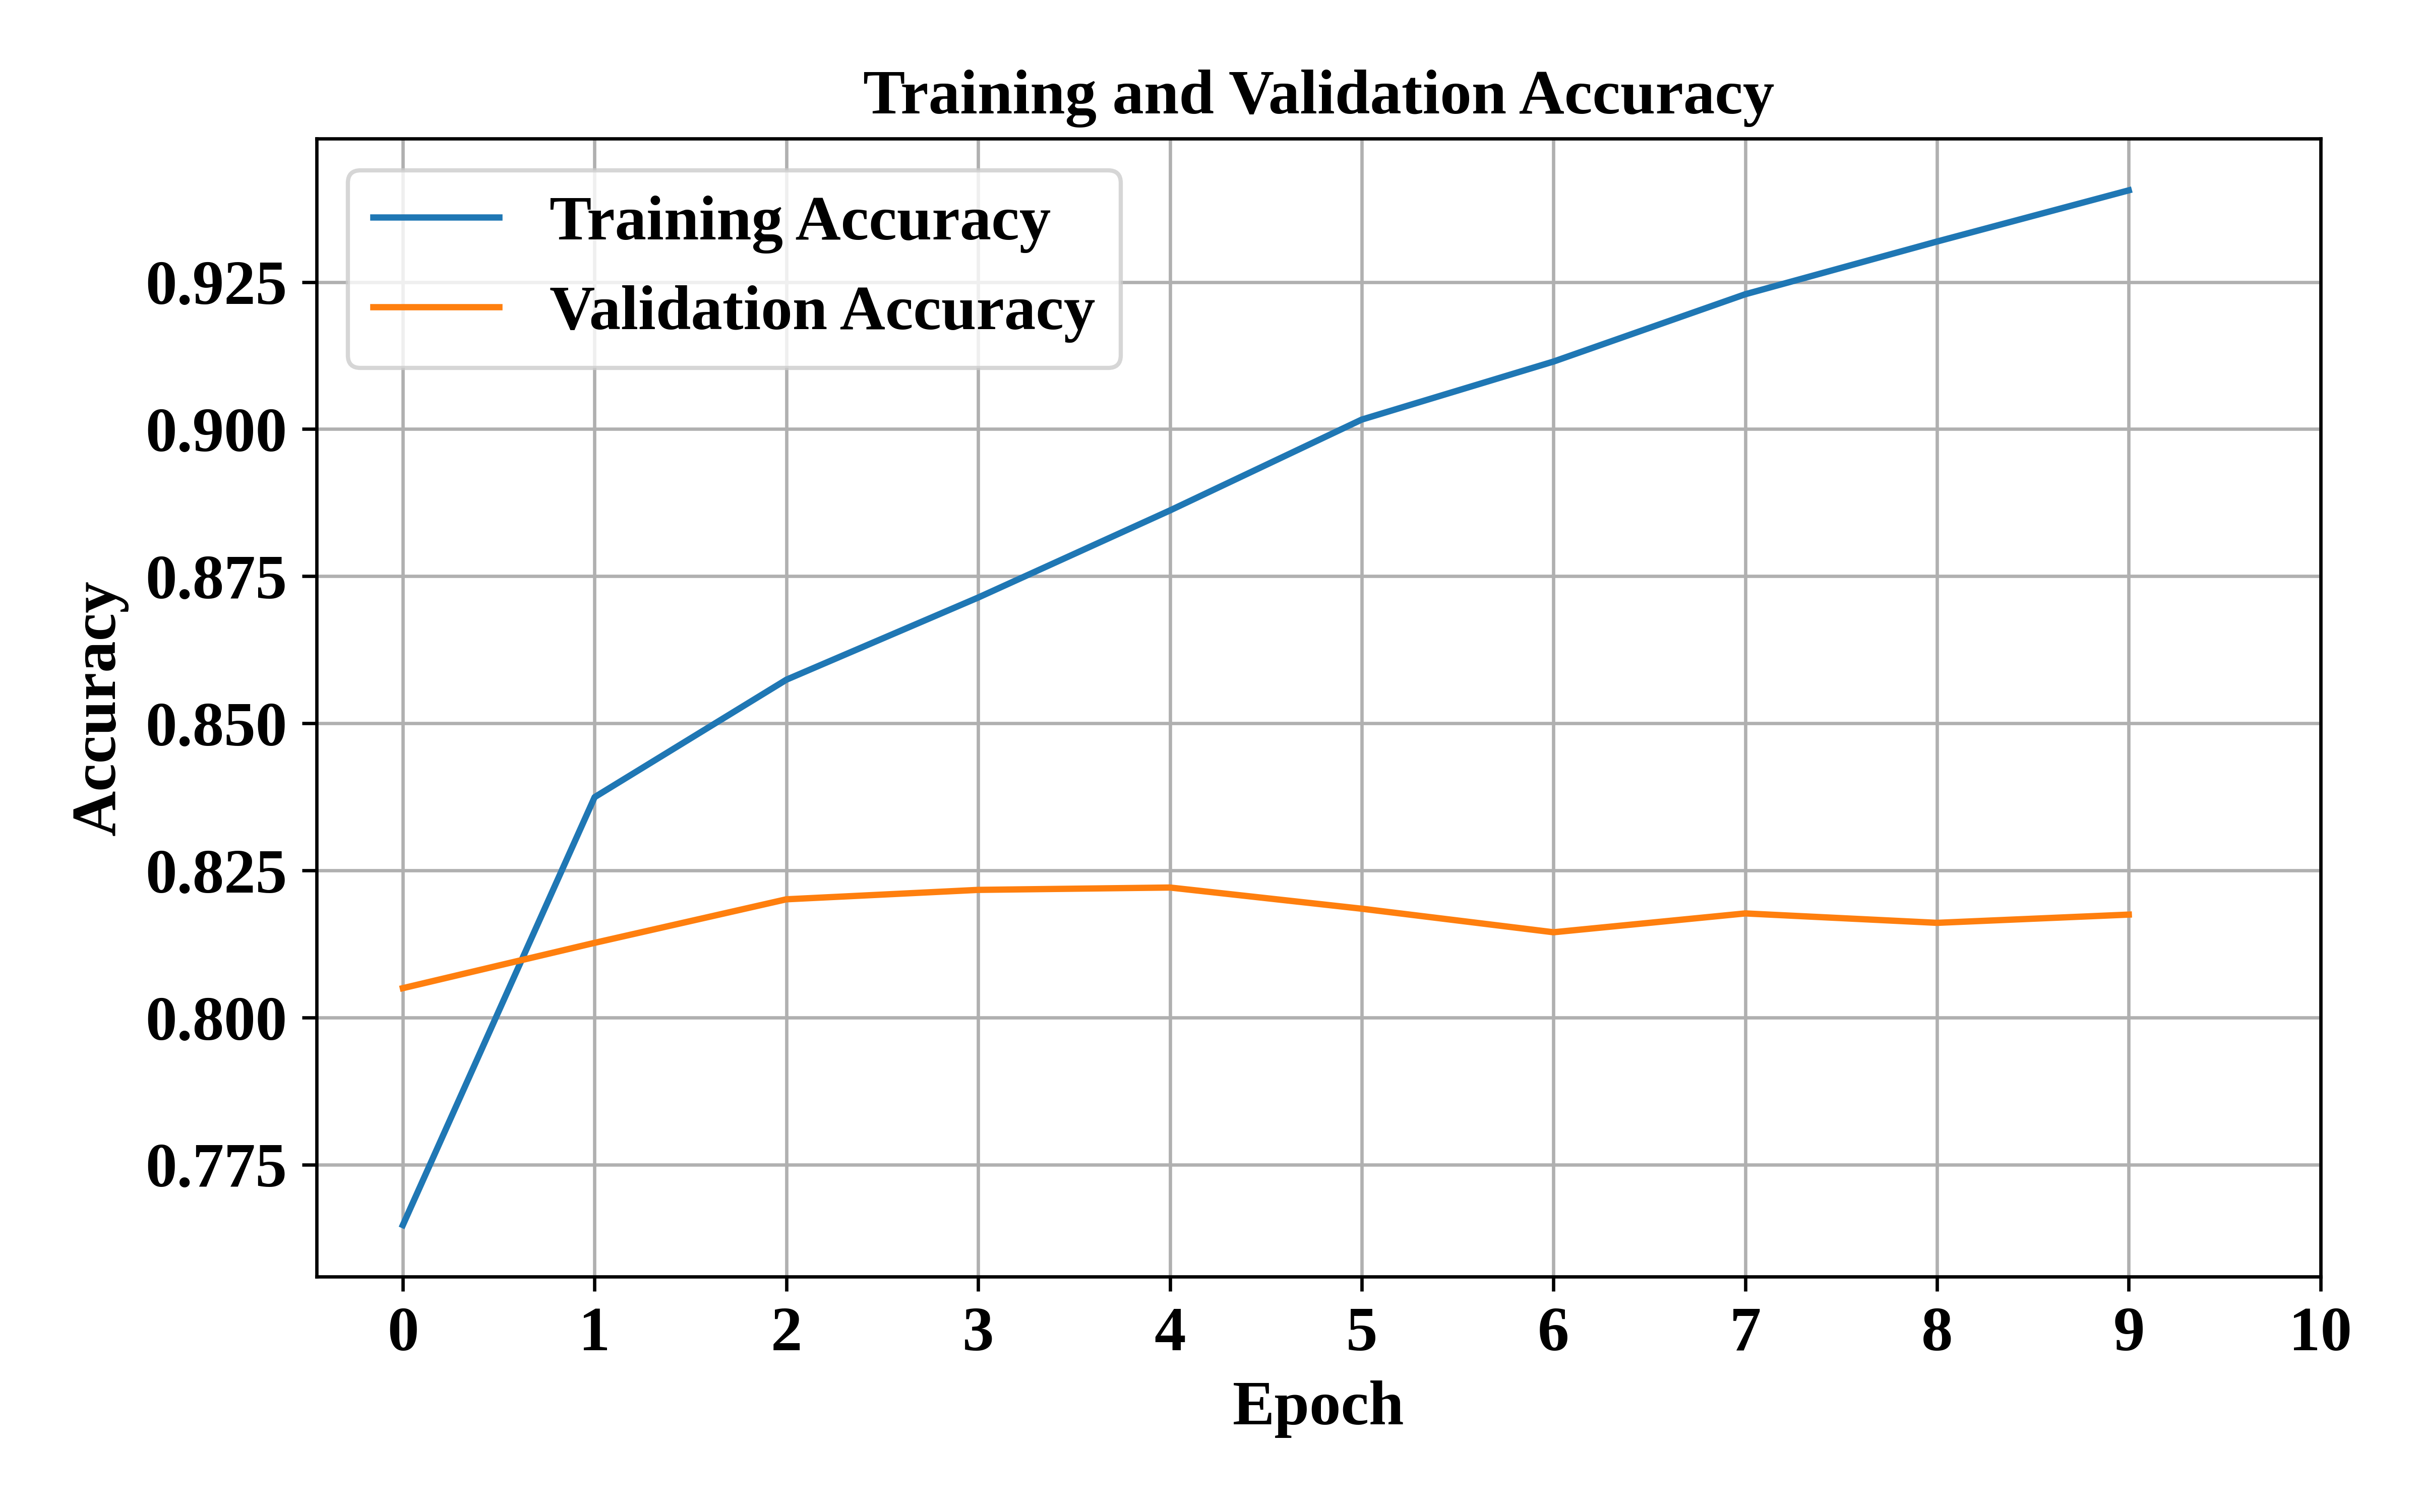
\includegraphics[width=0.9\textwidth]{Images/TrainValAccuracy.png}
            \caption{Training and Validation Accuracy}
            \label{fig:TrainValAccuracy}
        \end{figure}
        \noindent\textbf{Inference:}\\
    Training accuracy increases smoothly from approximately 76 percent at Epoch 0 to over 92 percent by Epoch 9. 
    This shows that the model effectively fits the training data with subsequent epochs.

    Validation accuracy rises initially from around 80 percent and reaches its peak at approximately 82.5 percent around Epoch 3–4,.
    After Epoch 4, the validation accuracy stabilizes.

    After Epoch 4, training accuracy continues to rise while validation accuracy drops slightly and stabilizes. This shows that the model is overfititng.
    
    \clearpage
    \item\textbf{Training and Validation Loss}
            \begin{figure}[H]
            \centering
            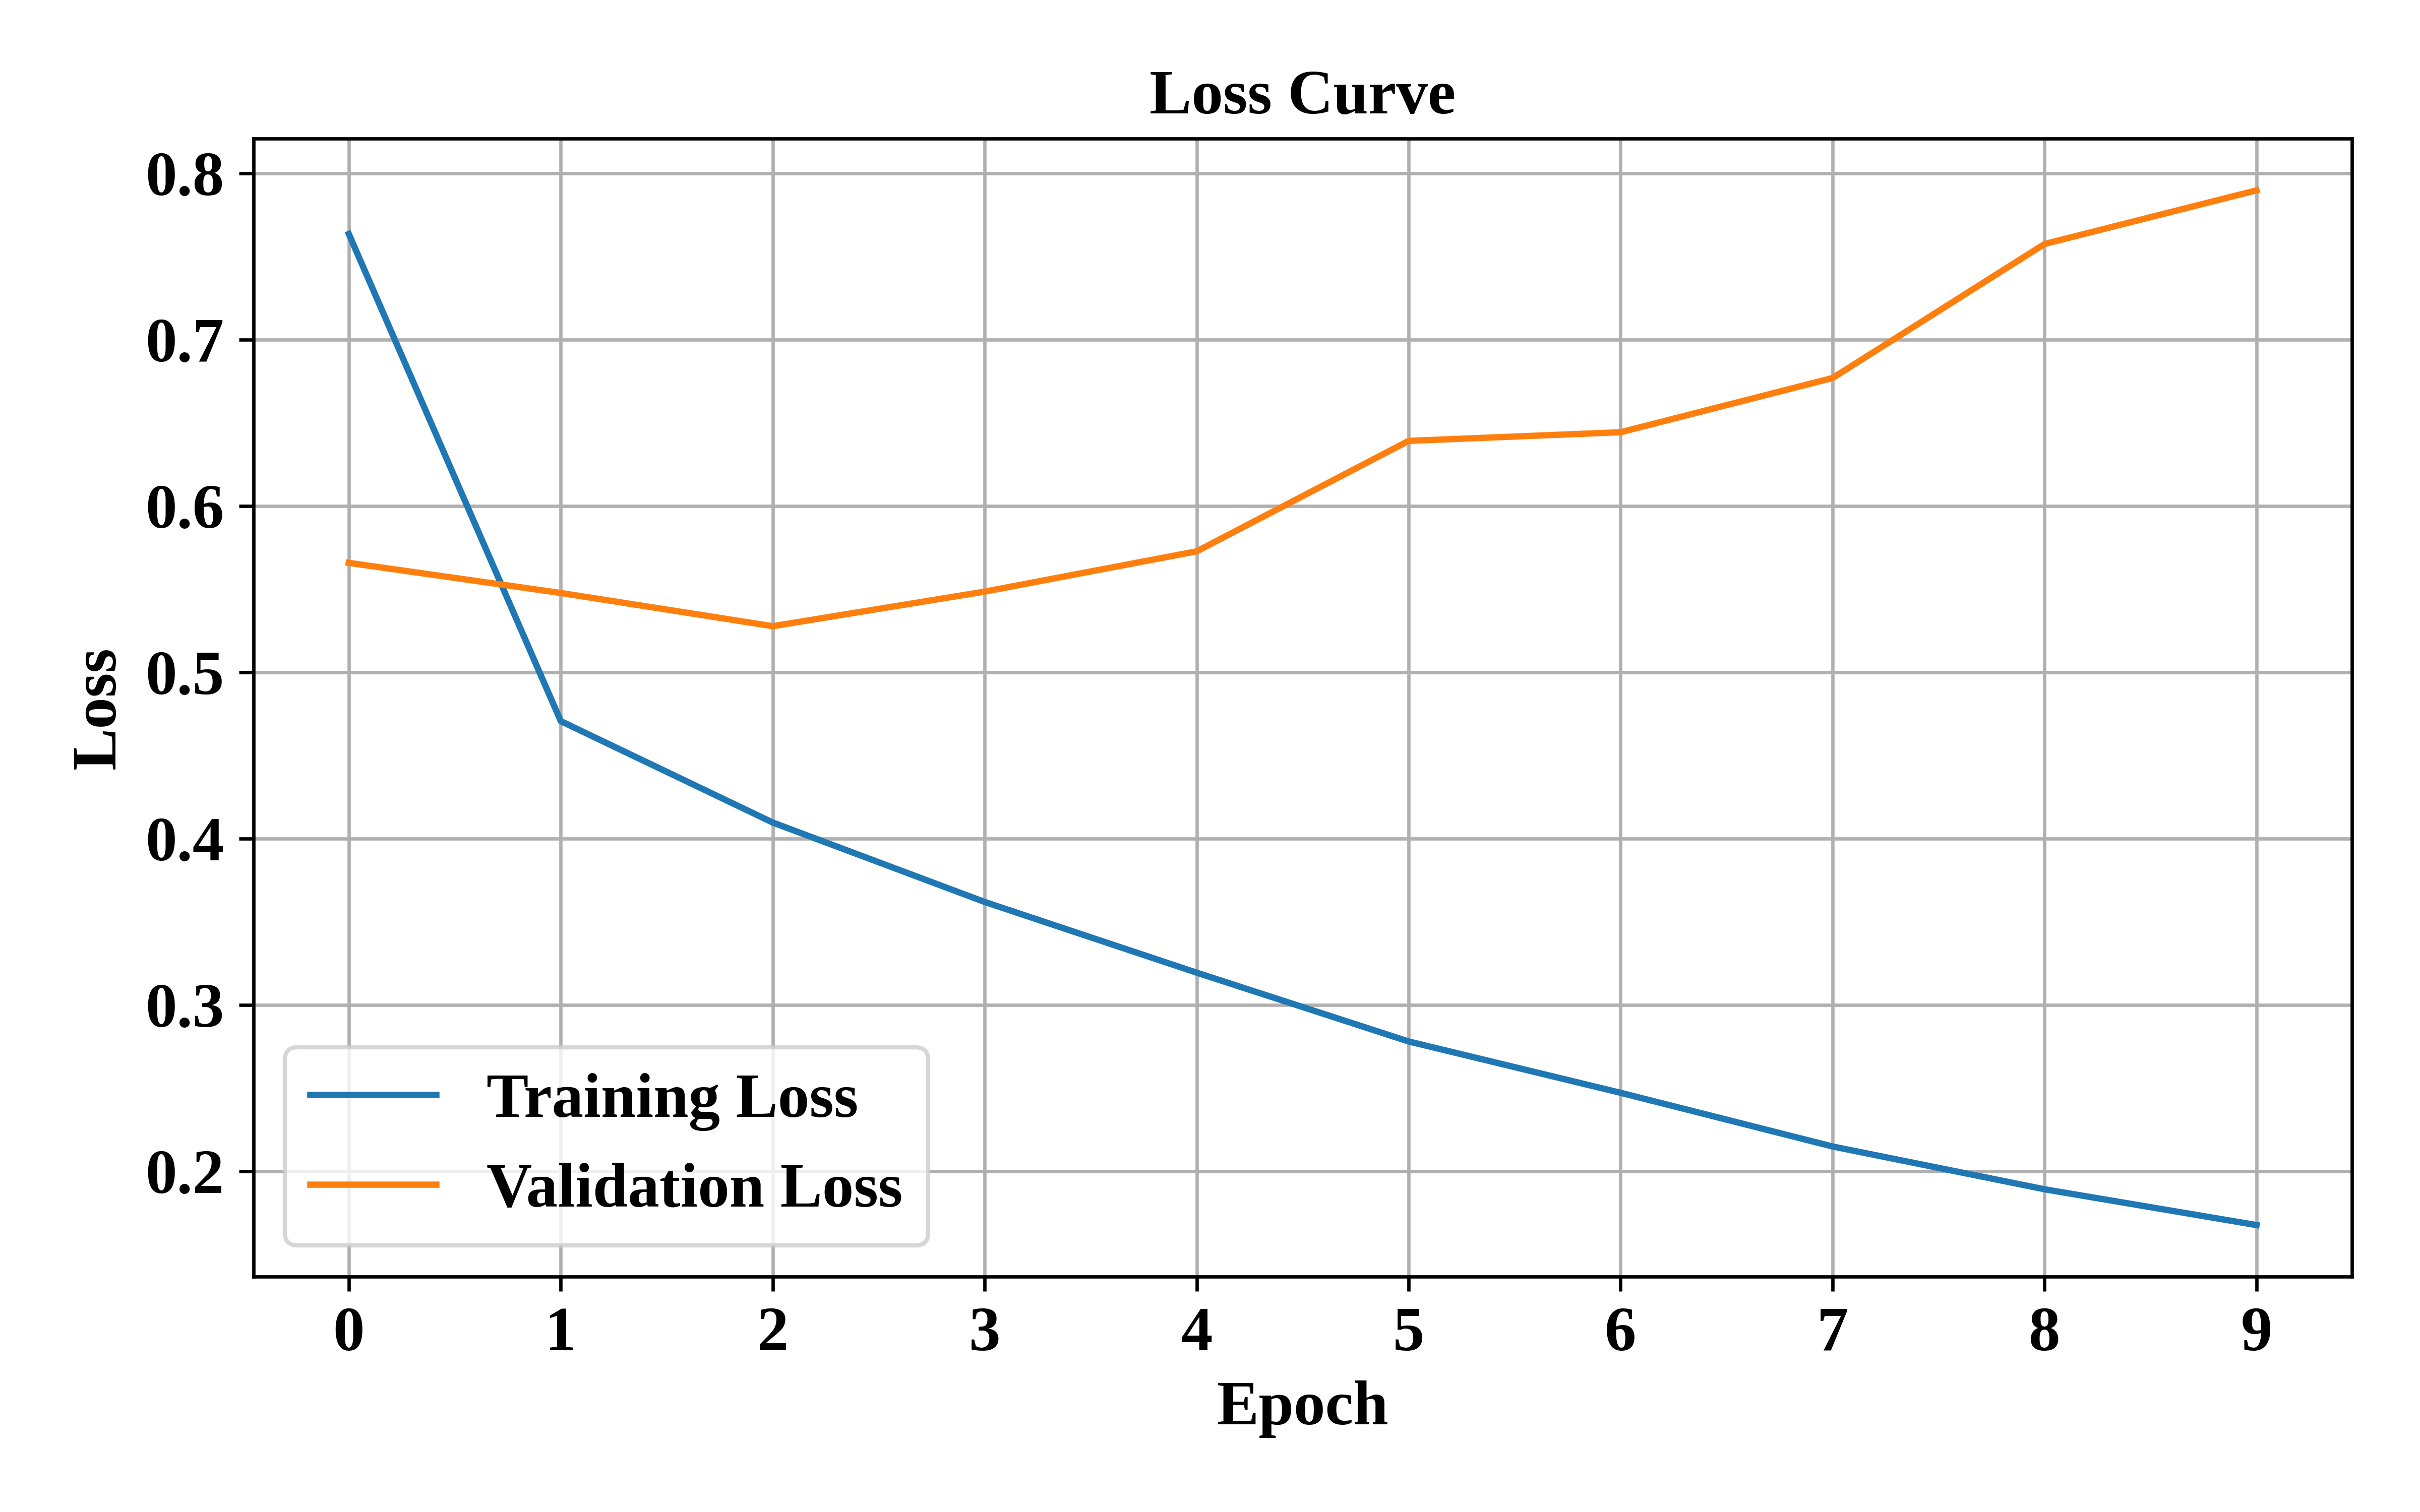
\includegraphics[width=0.9\textwidth]{Images/TrainValLoss.png}
            \caption{Training and Validation Loss}
            \label{fig:TrainValLoss}
        \end{figure}
        \noindent\textbf{Inference:}\\
    The training loss sharply decreases from 75 percent to around 0.5 percent within the first 2 epochs. 
    Then it steadily decreases for subsequent epochs.

    Validation loss decreases initially reaching its lowest point with value about 50 percent around Epoch 2.
    Then the validation loss increases.

    The gap between training and validation loss curves suggests that the model is learning the training data well but has limited generalization to unseen data.


    \clearpage
    \item\textbf{Confusion Matrix}
        \begin{figure}[H]
        \centering
        
\includegraphics[width=0.9\textwidth]{Images/ConfusionMatrix.png}
        \caption{Confusion Matrix}
        \label{fig:ConfusionMatrix}
    \end{figure}
    \noindent\textbf{Inference:}\\
    The confusion matrix shows that all the classes have been correctly classified most of the time.
    However 115 Dog images have been incorrecly classified as Cat. Also 67 Cat images have been incorrectly classified as Dog.
    In addition, 43 Airplane images have been misclassified as Ship. Also 34 images of Automobile has been misclassified as Truck. 
    Moreover 36 Deer images has been misclassified as Horse.

    This shows that the model has been able to predict most of the classses very well. 
    However there is some misclassification among similar classes such as Dog and Cat, Deer and Horse, Automobile and Truck.

    \clearpage
    \item\textbf{Misclassified Images}
            \begin{figure}[H]
            \centering
            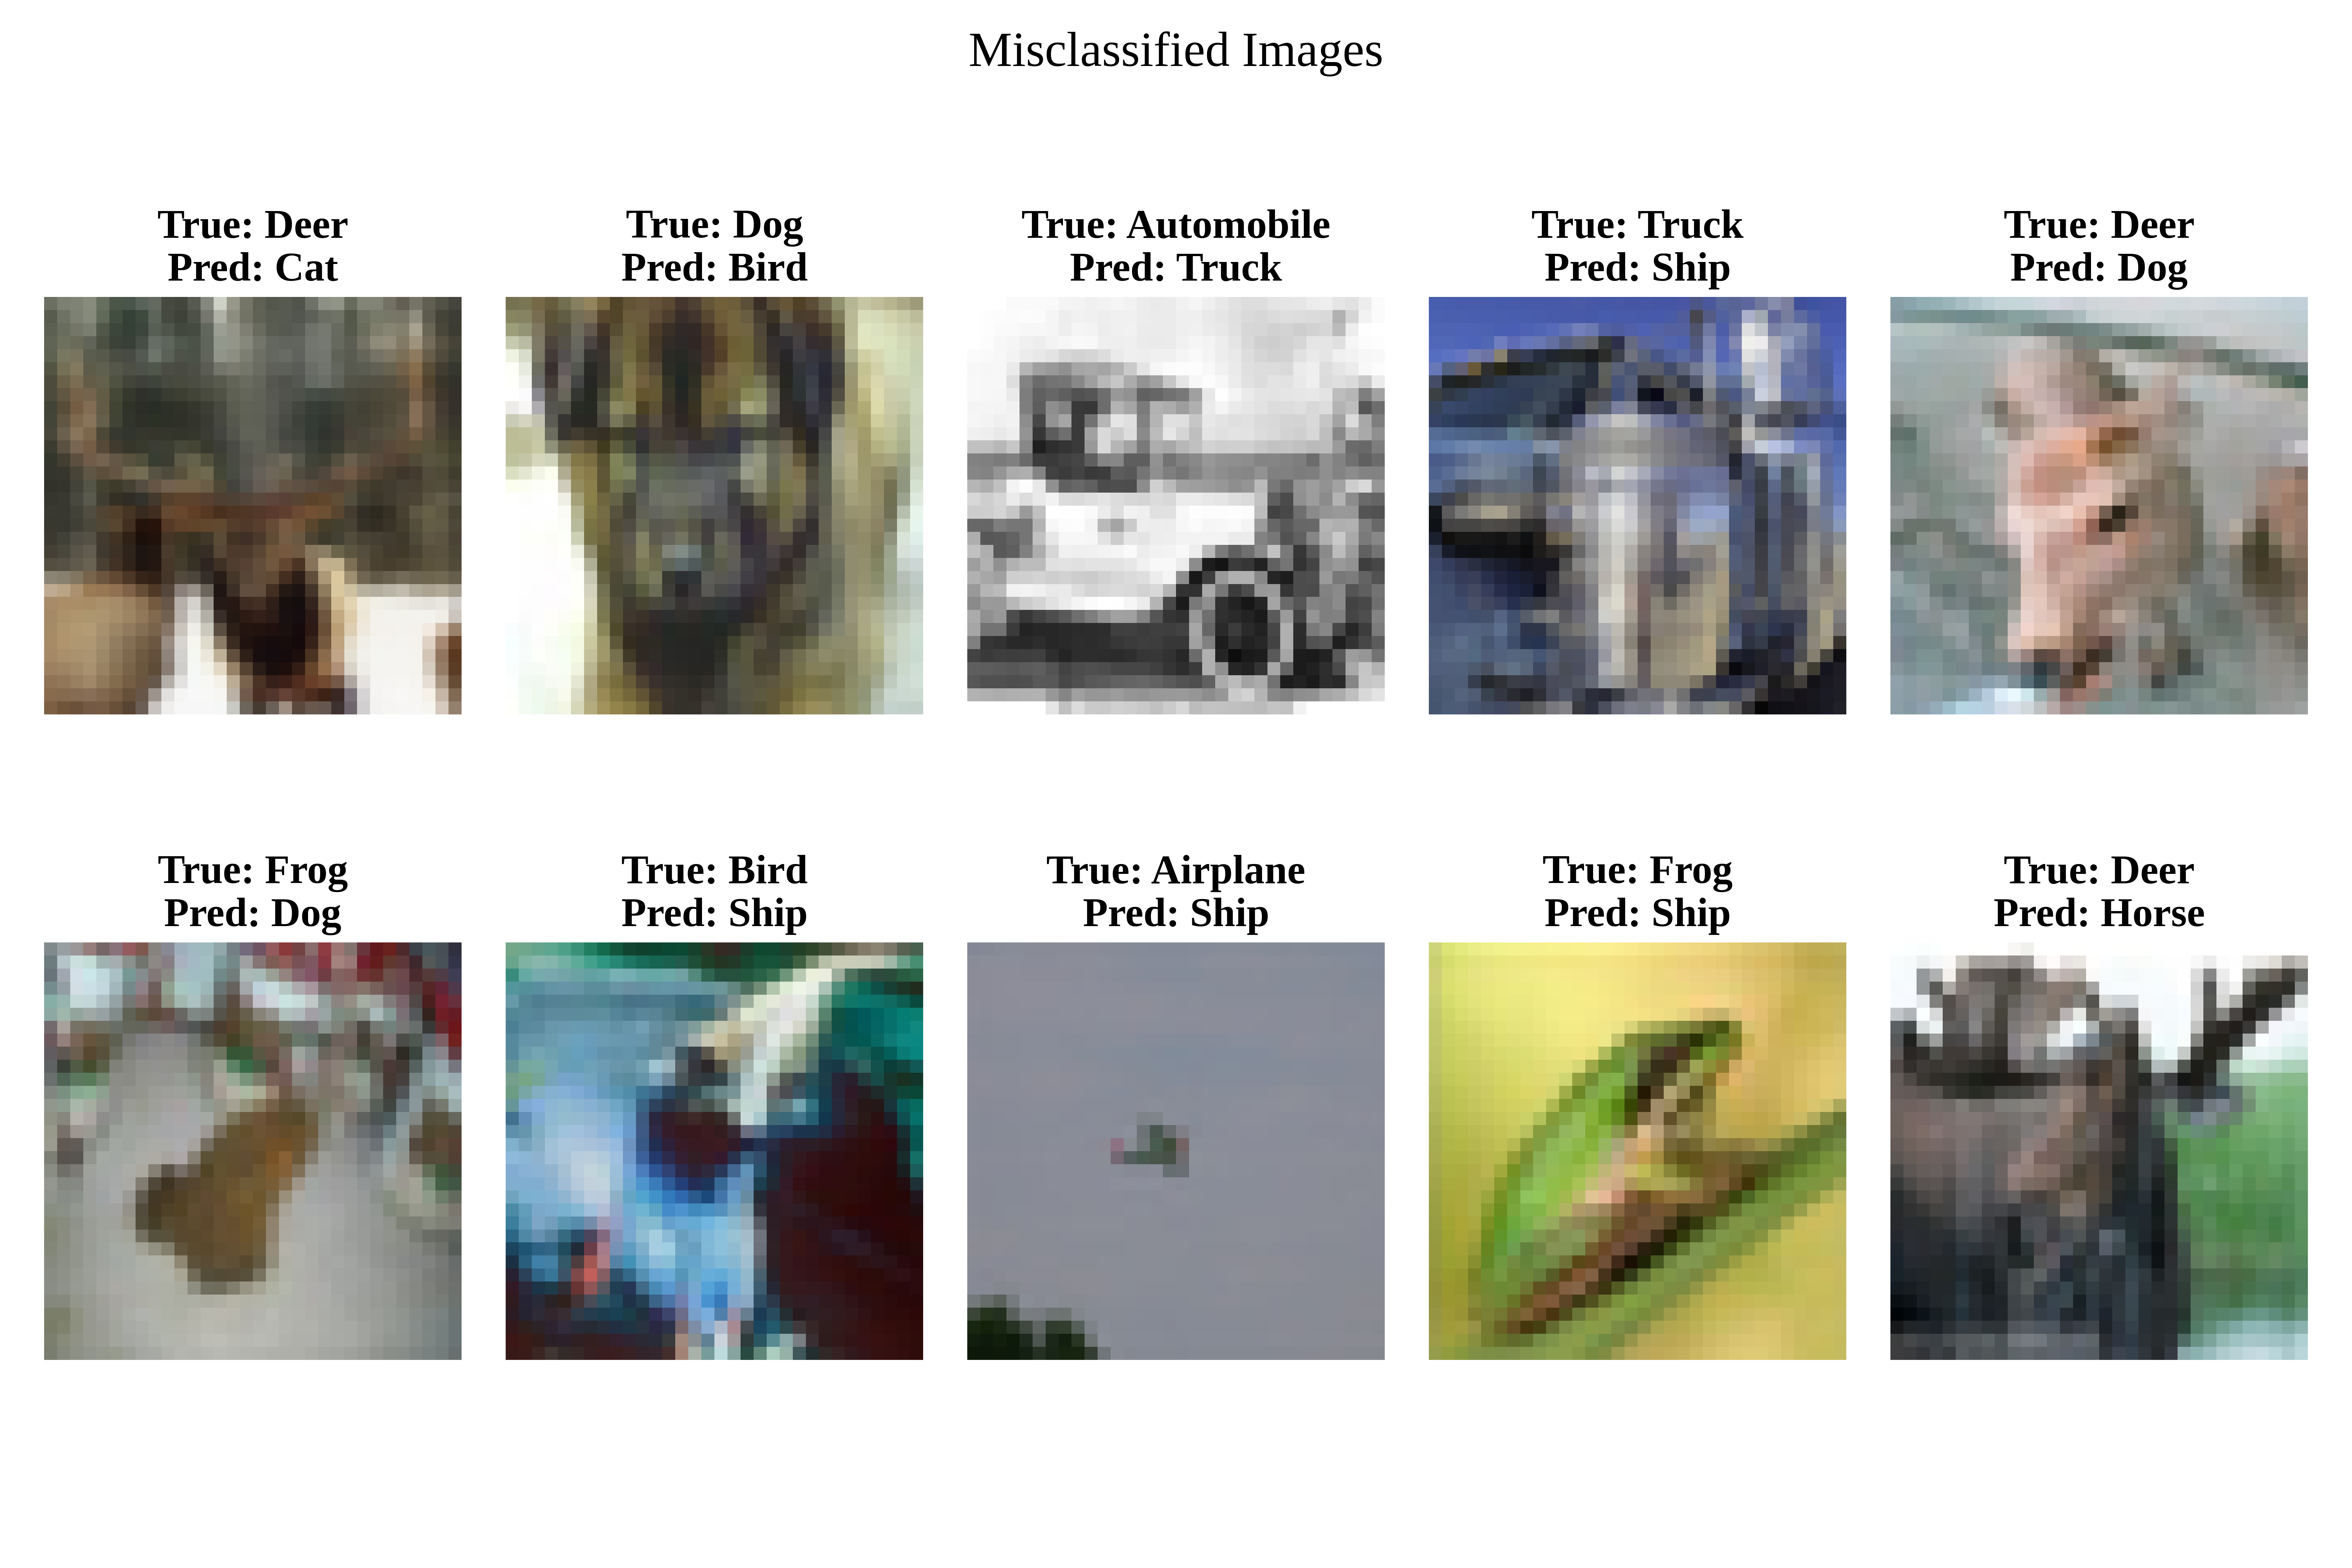
\includegraphics[width=0.9\textwidth]{Images/MisclassifiedImages.png}
            \caption{Misclassified Images}
            \label{fig:MisclassifiedImages}
        \end{figure}
        \noindent\textbf{Inference:}\\
    The figure shows some of the images that has been misclassified by the model.
    From this figure we can see that Deer image has been misclassified as Dog and Horse. 
    Similarly Frog image has been misclassified as Dog and Ship.
    
\end{enumerate}

\clearpage
\section{Results}

\subsection{Performance Metrics}
\begin{table}[H]
\centering
\begin{tabular}{|l|p{6cm}|}
\hline
\textbf{Metric} & \textbf{Value} \\ \hline
Training Accuracy &  0.9406 \\ \hline
Testing Accuracy & 0.9105 \\ \hline
Precision &  0.9124063566237557 \\ \hline
Recall & 0.9105 \\ \hline
F1-score &  0.9107742104848716 \\ \hline
Training Time & 769.273529291153 seconds\\ \hline
Total Parameters & 29,074,400 \\ \hline
\end{tabular}
\end{table}

\subsection{Comparison of CNN Architectures}
\begin{table}[H]
\centering
\begin{tabular}{|l|l|l|l|}
\hline
\textbf{Model} & \textbf{Parameters} & \textbf{Accuracy (\%)} & \textbf{Training Time} \\ \hline
LeNet-5 & 83,126 & 54.45 & 77.5 seconds\\ \hline
AlexNet & 36,925,322 & 71.19	& 343.1 seconds\\ \hline
VGG16 & 29,074,400 & 91.05 & 769.3 seconds \\ \hline
GoogleNet & 22,066,346 & 69.58 & 296.1 seconds \\ \hline
ResNet50 & 23,851,274 & 86.38 & 392.7 seconds\\ \hline
\end{tabular}
\end{table}

\subsection{Hyperparameter Study}
\textbf{VGG16}
\begin{table}[H]
\centering
\resizebox{\textwidth}{!}{%
\begin{tabular}{|l|l|l|l|l|l|l|l|}
\hline
\textbf{Learning Rate} & \textbf{Batch Size} & \textbf{Epochs} & \textbf{Optimizer} &
\textbf{Dense Units} & \textbf{Frozen} & \textbf{Validation Accuracy} & \textbf{Time (sec)} \\
\hline
0.001 & 32 & 10 & Adam & 128 & All & 0.8216 & 769.60 \\
\hline
0.0001 & 32 & 10 & Adam & 128 & All & 0.8197 & 776.33 \\
\hline
0.001 & 16 & 10 & Adam & 128 & All & 0.8195 & 772.22 \\
\hline
0.001 & 64 & 10 & Adam & 128 & All & 0.8219 & 711.69 \\
\hline
0.001 & 32 & 20 & Adam & 128 & All & 0.8248 & 1527.30 \\
\hline
0.001 & 32 & 10 & SGD & 128 & All & 0.8018 & 767.58 \\
\hline
0.001 & 32 & 10 & Adam & 256 & All & 0.8230 & 767.40 \\
\hline
0.001 & 32 & 10 & Adam & 128 & Partial & 0.1000 & 1001.75 \\
\hline
\end{tabular}%
}
\end{table}

\clearpage
\section{Discussion Questions}
Answer the following questions:
\begin{enumerate}[leftmargin=*]
    \item \textbf{Why is AlexNet considered a breakthrough in deep learning?}
    
    \vspace{5mm}
    
    AlexNet was a major breakthrough because it demonstrated that a deep convolutional neural network (CNN) could achieve better performance on large-scale image classification.
    It used techniques like ReLU, dropout, data augmentation, and GPUs for faster training.
    
    \vspace{3mm}
    
    \item \textbf{Why does VGG16 use only $3 \times 3$ convolution filters?}
    
    \vspace{5mm}
    
    VGG16 uses 3 x 3 convolution filters because they require fewer parameters and computations than larger filters.
    Stacking two 3 x 3 filters gives an effective 5 x 5 receptive field, wheras stacking three 3x3 filters gives a 7 x 7 receptive field.
    This allows the network to capture larger patterns without using large filters directly.
    Each convolution is followed by ReLU, providing more nonlinearities and helping the network learn complex features.
    Using small filters also allows VGG16 to build a deeper network.
    Thus, 3 x 3 filters provide better feature learning with fewer parameters and greater depth.
    
    \vspace{3mm}
    
    \item \textbf{Explain the advantages of the Inception module.}
    
    \vspace{5mm}
    
    The Inception module processes an image using different operations like 1x1, 3x3, 5x5 convolutions and pooling in parallel.
    It can capture features at different scales, from small details to larger patterns.
    The outputs of these branches are combined to create a richer feature representation.
    Using 1x1 convolutions reduce the number of channels which lowers computational cost.
    Thus, Inception provides better feature extraction and computational efficiency.
    
    \vspace{3mm}
    
    \item \textbf{What is the purpose of residual learning?}
    
    \vspace{5mm}
    
    The main purpose of residual learning is to make very deep neural networks easier and more effective to train.
    Instead of learning the entire transformation, the network learns only the difference (residual) between the input and the desired output.
    Skip connections allow the original input to directly reach later layers, helping information and gradients flow smoothly.
    This helps prevent problems such as vanishing gradients and degradation, where adding more layers can actually reduce performance.
    It also makes the network easier to optimize because the layers only need to learn the necessary changes.
    Residual learning allows models like ResNet to become very deep while still maintaining good performance.
    
    \vspace{3mm}
    
    \item \textbf{Differentiate LeNet and ResNet.}
    
    \vspace{5mm}
    
    LeNet is a simple and shallow CNN mainly designed for handwritten digit recognition.
    On the other hand, ResNet is a much deeper CNN designed for complex image classification tasks.
    LeNet does not use skip connections, while ResNet can skip connections.
    LeNet has fewer parameters and requires less computation.
    Whereas, ResNet can have 18, 34, 50, 101, or 152 layers, making it much more powerful but computationally expensive.
    
    \vspace{3mm}
    
    \item \textbf{What is Transfer Learning?}
    
    \vspace{5mm}
    
    Transfer Learning is the process of using a model already trained on a large dataset for a new similar task.
    The pretrained model already knows useful features such as edges, textures, and shapes.
    These learned features are used instead of training a model from scratch.
    Here, the final classification layer is replaced according to the new task.
    It helps reduce training time, data requirements, and computational cost.
        
    \vspace{3mm}
    
    \item \textbf{Why is fine tuning required?}
    
    \vspace{5mm}
    
    Fine-tuning is used to adapt a pretrained model to a new task.
    A pretrained model already knows general features like edges, shapes, and textures, but it may not understand the specific features of the new task.
    Here we unfreeze some of the deeper layers and train them with the new data.
    A small learning rate is usually used so that the useful features already learned are not lost.
    This helps the model achieve better accuracy with less training time.
    
    \vspace{3mm}
    
    \item \textbf{Explain the difference between dilated convolution and transpose convolution.}
    
    \vspace{5mm}
    
    Dilated convolution increases the receptive field by adding gaps between kernel elements.
    It captures information from a larger area without greatly increasing the number of parameters.
    Transpose convolution is mainly used to increase the spatial size of feature maps.
    Dilated convolution is commonly used in segmentation, while transpose convolution is used in decoders and image generation.
    
    \vspace{3mm}
    
    \item \textbf{Why do pretrained models converge faster?}
    
    \vspace{5mm}
    
    Pretrained models start with already learned weights instead of random weights.
    They already know useful features such as edges, textures, shapes, and patterns.
    Therefore, the model does not need to learn these features from the beginning.
    It only needs to adapt the existing features to the new dataset or task.
    As a result, pretrained models generally require fewer epochs and less training time to achieve good performance.
    
    \vspace{3mm}
    
    \item \textbf{Compare the computational complexity of LeNet and ResNet.}
    
    \vspace{5mm}
    
    LeNet is a small and simple CNN with fewer layers and parameters so it requires less computation.
    ResNet is much deeper and has many more layers and parameters so it needs more computational power.
    As a result, ResNet requires more mathematical calculations, memory, and training time than LeNet.
    LeNet is lightweight and fast. Hence it can run easily on basic hardware. 
    However ResNet is computationally expensive and works better with a GPU.    
    \vspace{3mm}
    
\end{enumerate}

\clearpage
\section{Additional Exercises}
\begin{enumerate}[leftmargin=*]
    \item Implement transfer learning using VGG16.
    \item Repeat the experiment using ResNet50.
    \item Compare Adam and SGD optimizers.
    \item Compare training with frozen layers and fine tuning.
    \item Evaluate the model using Precision, Recall and F1-score.
    \item Compare the performance of LeNet, AlexNet and ResNet.
\end{enumerate}

\section{References}
\begin{enumerate}[leftmargin=*]
    \item Yann LeCun, Leon Bottou, Yoshua Bengio and Patrick Haffner, \textit{Gradient-Based Learning Applied to Document Recognition}, Proceedings of the IEEE, 1998.
    \item Alex Krizhevsky, Ilya Sutskever and Geoffrey Hinton, \textit{ImageNet Classification with Deep Convolutional Neural Networks}, NeurIPS, 2012.
    \item Karen Simonyan and Andrew Zisserman, \textit{Very Deep Convolutional Networks for Large-Scale Image Recognition}, ICLR, 2015.
    \item Christian Szegedy et al., \textit{Going Deeper with Convolutions}, CVPR, 2015.
    \item Kaiming He, Xiangyu Zhang, Shaoqing Ren and Jian Sun, \textit{Deep Residual Learning for Image Recognition}, CVPR, 2016.
    \item Ian Goodfellow, Yoshua Bengio and Aaron Courville, \textit{Deep Learning}, MIT Press, 2016.
    \item TensorFlow Documentation: \url{https://www.tensorflow.org}
    \item Keras Documentation: \url{https://keras.io}
\end{enumerate}

\end{document}